\chapter{Neural Networks}
The brain has been studied deeply during the last century. The researchers wanted to use the power of the brain in a mathematical or computational model. The first step in the Deep Learning was to copy the behaviour of the brain neurons to a circuit (1943, neurophysiologist Warren McCulloch and mathematician Walter Pitts). The poor computing capacity of the time stopped the studies on the topic.\\

In the 80s the field became again interesting with the inclusion of multiple layered neural networks. In 1986 researchers modeled the idea of back propagation. This idea helps the network to distribute pattern recognition errors throughout the whole network. The problem is that with this algorithm the net learn slowly, so many iterations are needed. \\

Nowadays Neural Networks are incredibly important. The big data and the computing capacity are a perfect base for the networks. Also with new types of models such as Convolutional Neural Networks or Recurrent Neural Networks they are solving amazing problems beyond the image recognition. \cite{hnet1} \cite{hnet2}

\section{What is a Neural Network}
You could think of a Neural Network as a box with a certain number of inputs and outputs. For a given input the box answer with a output, that is the network prediction.

Let us imagine that we have one box of this kind, and if you input a image of a handwritten digit, the output of the box will be the digit of the picture. You could think that if you create one box like this you have all your work done, but the box by itself is stupid. If you create a box and feed it with the picture of a '1' the output could be whatever.

What we should do is to teach the net so it could answer correctly. To achieve it our box has several knobs that we can regulate in order to tell the box how bad was the prediction it said. In that way, after correcting the knobs several times, the box has learned, what means that it is ready for answer right. Now we have a box with the knowledge to make good predictions, but since it is a box we cannot outcome any knowledge for us. We cannot get any method to create an algorythm that solve our task more efficiently. We just can use our box, and get our answer from our box.


\section{Under the Hood}
\label{sec:hood}
Now that we have understood our box it is time to start knowing what is inside it. The neural network is composed by several layers. At least we have the input layer (receive the data from outside) and the output layer (give us the prediction). Between those two could be more hidden layers. Each of them has a certain number of neurons $n_1, n_2, .., n_m$ where $m$ is the number of layers. That means that the input layer has $n_1$ neurons while the output layer has $n_m$ neurons. Each neuron of the first layer is connected with each neuron of the second layer, each neuron of the second layer is connected with each neuron of the third layer and so on (See Figure ~\ref{fig:net2}). \\

\begin{figure}
  \center
  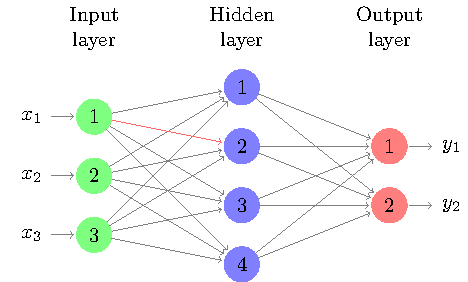
\includegraphics[scale=1.5]{images/net2.pdf}
  \caption{\label{fig:net2}Example of Neural Network with 3 layers. Here $n_1=3$, $n_2=4$ and $n_3=2$. The connection in red is denoted as $w^{(1)}_{12}$ (according to Equation ~\ref{eq:w})}
\end{figure}

Each of those connections has a weight $w$. To denote these weights we are going to use the form $w_{ij}^{(k)}$ where $k$ means which layer the connection departs from, $i$ means which neuron of layer $k$ the connection departs from and $j$ means which neuron of layer $k+1$ the connections arrives to (See Figure ~\ref{fig:net2}). Therefore $w$ is:
\begin{equation}
\begin{aligned}
  & w^{(k)}_{ij} \\
  & i=1,\dots,n_k \\
  & j=1,\dots,n_{k+1} \\
  & k=1,\dots,m
\end{aligned}
\label{eq:w}
\end{equation}\\

Each neuron has a bias that allow set how excited is a neuron. A really excited neuron always output '1' while a non-excited neuron always give us '0'. The bias helps the network to adjust some neurons as important since not every neuron output is equally interesting. The work of a single neuron is as simple as add the bias and the weighted inputs and apply a function to the result ~\cite[Chapter~27]{springer}. The output $o$ of a neuron is:
\begin{equation}
  o^{(k)}_i=
  \begin{cases}
    x_i, & k=1 \\
    f\bigg(u^{(k)}_i+\sum^{n_{k-1}}_{j=1}w^{(k-1)}_{ji}\cdot o^{(k-1)}_j\bigg), & k>1
  \end{cases}
\end{equation}
For example, for the neuron 3 in blue of Figure ~\ref{fig:net2} the output will be $o^{(2)}_3=f(u^{(2)}_3+w^{(1)}_{13}\cdot o^{(1)}_1+w^{(1)}_{23}\cdot o^{(1)}_2+w^{(1)}_{33}\cdot o^{(1)}_3)$. For the same neuron the scheme is showed in Figure ~\ref{fig:neur1}.
\begin{figure}[H]
  \center
  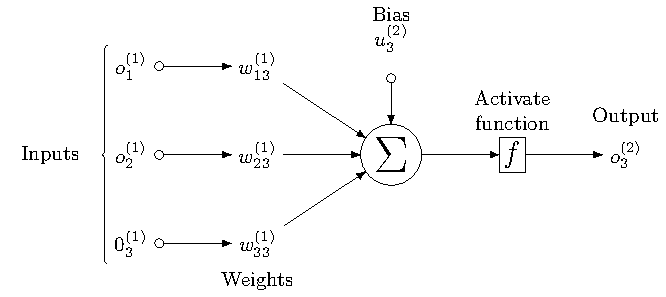
\includegraphics[scale=1]{images/neuron1.pdf}
  \caption{\label{fig:neur1}Example of the task of a single neuron \cite{neurdiag}}
\end{figure}

\section{Back Propagation}
Now a Neural Network could be programmed with all showed on \ref{sec:hood}, a program that output $y_1,$ and $y_2$ could be developed. But, where is the "learning" of deep learning here? Nowhere, yet. Is the moment of teaching the net with examples, giving it some inputs and showing it the expected outputs. The \textit{Back Propagation Algorithm} is going to achieve it. The goal of this method is to minimize the error using the method of gradient descent.

\subsection{Activation Function}
As explained before each neuron has to apply one function to the result of its computing. One of the most popular functions used for this purpose is the sigmoid:
\begin{equation}
  s(x)=\frac{1}{1+e^{-cx}}
\end{equation}
The shape of this function depends on the value of $c$, but for simplicity $c=1$ is going to be used. The derivate of the sigmoid function respect of x is $s(x)^\prime=s(x)(1-s(x))$. One of the reasons why this function is used is the simplicity of the derivate, because it allows to make all the derivates later more easily ~\cite[Chapter~7]{rojas}.
\begin{figure}
  \center
  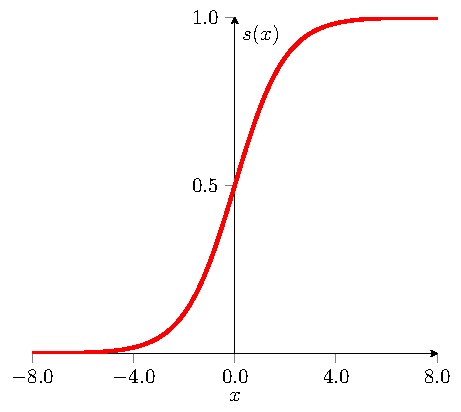
\includegraphics{images/sigmoid.pdf}
  \caption{Shape of the sigmoid with $c=1$}
\end{figure}

\subsection{The Error}
The error could be measured in differents ways. The most common and apparently most effective method is to calculate the Euclidean distance. It allows to measure the error in different dimensions, for example, the error in $\rm I\!R^1$ between $4$ and $1$ is $E=4-3=1$. For $\rm I\!R^2$ you should use the Pythagorean theorem, and for $\rm I\!R^n$ the distance is:
\begin{equation}
  E_{(p,q)}=\sqrt{(p_1-q_1)^2+(p_2-q_2)^2+\dots+(p_i-q_i)^2+\dots+(p_n-q_n)^2}
\end{equation}

Is important to know how to size the error that the net has because you have to tell the network how far was the result from the expected output. And only once you have the distance between the target and the output you can adjust the knobs to achieve a better result.

How much the knob must be changed? It depends on how important is that knob for the result. For example it might be possible that changing one knob will get the same result. In this case it does not matter if we adjust the knob, but, what about one knob that when adjusted change the result drastically? Here the new position of the knob is realy important. Hence we need the partial error with respect a specific weight or bias ~\cite[Chapter~2]{nielsen}:
\begin{equation}
  \frac{\partial e}{\partial w^{(k)}_{ij}} \quad \textrm{or} \quad \frac{\partial e}{\partial u^{(k)}_{i}}
\end{equation}

\subsection{The Correction}
Once we can calculate the error depending on one parameter we are ready to make the correction to the network. The process is simple, first you feed the input layer with some data, then you get the result and compare it with the target and finally you make this adjustment for each weight and bias (the $\alpha$ is the learning constant and represent how far is the next step in the gradient descent) ~\cite[Chapter~7]{rojas}:
\begin{equation}
\begin{aligned}
  w^{(k)}_{ij} & \Rightarrow & w^{(k)}_{ij} - \alpha \frac{\partial e}{\partial w^{(k)}_{ij}} \\
  u^{(k)}_{i} &  \Rightarrow & u^{(k)}_{i} - \alpha \frac{\partial e}{\partial u^{(k)}_{i}}
\end{aligned}
\label{eq:corr}
\end{equation}

To develop a working neural network is now possible with all this knwoledge. First we have to declare the architecture of our net. Then we set random weights and biases and we start teaching the net. Imagine you have a 10.000 images dataset, then you take 90\% of those images to train the net, and the other 10\% for testing how well we have developed it. We feed the network with one of those images from the train set and make the correction as we have seen in \ref{eq:corr}. Ideally we should do it with all the train set but as the size of that set could be (and should be) huge, we just take a small batch representative and apply the correction for each image of the batch. Once we have done it we have complete one epoch. With just one epoch the network still giving us weird answers, so what we have to do is to train the network with several epochs and then our network is trained and ready.

To measure how intelligent our network is you can use the test set of images to calculate the accuracy.

